% Created 2022-08-31 Wed 15:32
% Intended LaTeX compiler: pdflatex
\documentclass[10pt]{beamer}
\usepackage[utf8]{inputenc}
\usepackage[T1]{fontenc}
\usepackage{graphicx}
\usepackage{longtable}
\usepackage{wrapfig}
\usepackage{rotating}
\usepackage[normalem]{ulem}
\usepackage{amsmath}
\usepackage{amssymb}
\usepackage{capt-of}
\usepackage{hyperref}
\usepackage{minted}
\usepackage[T1]{fontenc}
\usepackage{pmboxdraw}
\usetheme{Berkeley}
\usefonttheme{professionalfonts}
\usepackage{booktabs}
\definecolor{mycolor}{rgb}{0.54706, 0.13725, 0.26667}
\usecolortheme[named=mycolor]{structure}
\setlength{\parskip}{5pt}
\newcommand{\footnoteframe}[1]{\footnote[frame]{#1}}
\addtobeamertemplate{footnote}{}{\vspace{2ex}}
\usepackage{xcolor}
\definecolor{LightGray}{gray}{0.95}
\usepackage{fancyvrb}
\DefineVerbatimEnvironment{verbatim}{Verbatim}{fontsize=\scriptsize}
\DeclareGraphicsRule{.gif}{png}{.png}{`convert #1 `dirname #1`/`basename #1 .gif`-gif-converted-to.png}
\DeclareGraphicsExtensions{.gif}
\usepackage{animate}
\usetheme{default}
\author{Jay Morgan}
\date{<TODO>}
\title{Machine Learning}
\subtitle{Lecture 2 - Linear Models}
\hypersetup{
 pdfauthor={Jay Morgan},
 pdftitle={Machine Learning},
 pdfkeywords={},
 pdfsubject={},
 pdfcreator={Emacs 28.1 (Org mode 9.5.4)}, 
 pdflang={English}}
\begin{document}

\maketitle

\section*{Linear Regression}
\label{sec:orged16787}

\subsection*{Introduction to linear models}
\label{sec:org4a5a1b9}

\begin{frame}[label={sec:org58e4148}]{Linear models}
Having learnt a little about what it means to learn, we're going to look at our first
\emph{Machine Learning} algorithm, the staple for much of statistics, numeric prediction
using a linear model.
\end{frame}

\begin{frame}[fragile,allowframebreaks,label=]{What is a linear model?}
A linear model is a prediction (a response) to an input variable. We have the
following terms:

\begin{itemize}
\item Response/prediction -- the output of the model.
\item Dependant variable -- the variable upon which the prediction is being made.
\end{itemize}

For a linear model based on one dependant we have the following:

\[
y = w x + b
\]

where \(y\) is the response/output/prediction of the model, \(x\) is the dependant
variable, and \(w, b\) are the model parameters.

If we look at our linear model equation, we'll notice that it's the same equation for a straight line.

\begin{center}
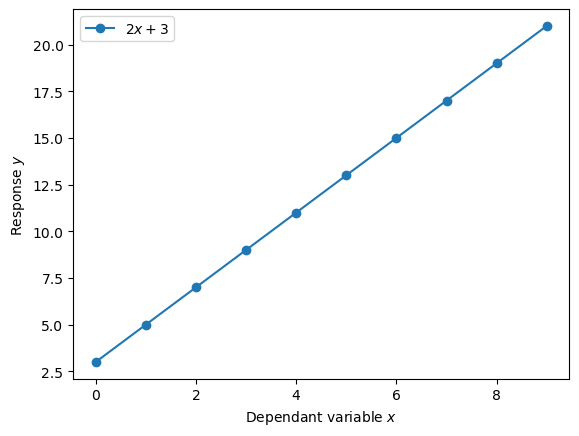
\includegraphics[width=.9\linewidth]{images/linear_model.png}
\end{center}
\end{frame}

\begin{frame}[label={sec:orgd367f10}]{Supporting example}
Let's have a look at how we would use this linear model with one of the datasets: The
Boston housing prices.

\begin{figure}[htbp]
\centering
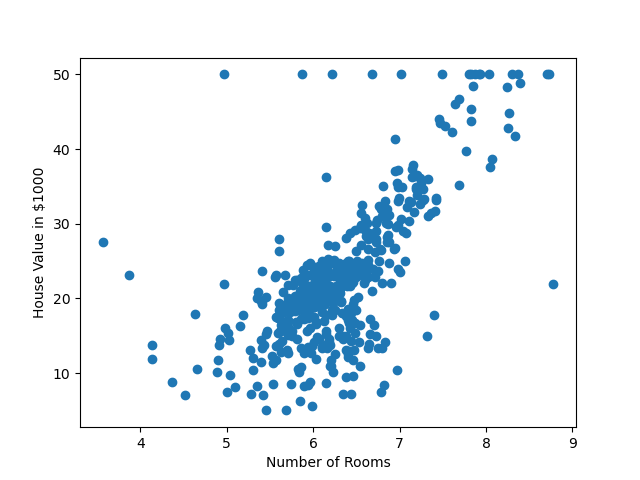
\includegraphics[width=0.6\textwidth]{images/boston_rooms_prices.png}
\caption{Scatter plot of the number of rooms in a house against the house valuation. In this plot we can see a positive effect with some outliers to this trend.}
\end{figure}
\end{frame}

\begin{frame}[fragile,allowframebreaks,label=]{Let's fit a linear model}
We have seen that there seems to be some correlation between the number of rooms and
the house price. I.e. we can use the number of rooms of the house to get the
estimated price. To get an estimated price we'll use our linear model:

\[
y = w x + b
\]

In this case, \(x\) will be the number of rooms. But what values should we set for \(w\)
and \(b\)? Or put another way, what is \emph{optimal} value for our model parameters.

We'll return to the question of optimal later, but for now, let's just select some
random values!

\[
w = 1
\]
\[
b = 1
\]

\begin{figure}[htbp]
\centering
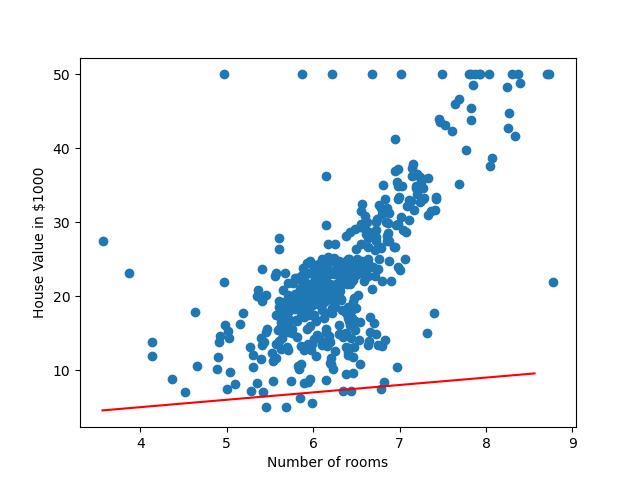
\includegraphics[width=.9\linewidth]{images/boston_rm_first_pred.png}
\caption{A linear model line overlayed onto the boston house prices dataset. Blue circles represent samples from the dataset, while the trend line is shown in red.}
\end{figure}

Well that doesn't look very good, it could be 'fit' better to what we're seeing in
the scatter plot! I wonder how wrong the linear model is -- how incorrect our
predicted house prices are?
\end{frame}

\begin{frame}[fragile,allowframebreaks,label=]{Evaluating our initial linear model}
To evaluate how well, or in this case, how badly our linear model is doing, let's
compare the predicted value from the model against the actual house price. For
example, we'll take a single sample from our dataset.

If we have 4 rooms, our model estimates the house price to be \(2(4) + 5 = 13\),
\$13,000, but the actual cost was \$24,000. This means we have underestimated the cost
by \$11,000.

What we've done there is the following:

\[
\delta = | y - \hat{y} |
\]

where \(\hat{y}\) is \(w x + b\)

We've calculated the difference or delta between the real house price \(y\) and the
predicted house price.

That gives us the error for one sample though, what about for the whole dataset? Well
we could take the mean over all samples:

\[
\Delta = \sum_{i=0}^n | y - \hat{y} |
\]

If we calculate that our linear model we see that the average difference between our
estimated value and real value is \$15,000!
\end{frame}

\begin{frame}[label={sec:orgfb90a7b}]{Loss curve}
\begin{itemize}
\item If we move the weight value, then we get a different point on the curve.
\end{itemize}
\end{frame}

\begin{frame}[label={sec:org6e55ae5}]{How to select the best weights}
\begin{itemize}
\item Lowest point on the curve.
\end{itemize}
\end{frame}

\begin{frame}[label={sec:org1985c21}]{Automatically computing the best weights}
\begin{itemize}
\item Gradient descent
\end{itemize}
\end{frame}

\section*{Logistic Regression}
\label{sec:org2c6d337}

\subsection*{Classification}
\label{sec:org0fa8076}

\begin{frame}[label={sec:org9676b11}]{Moving from regression to classification}
We now turn to classification
\end{frame}
\end{document}
